\documentclass[]{article}
\usepackage[UTF8]{ctex}
\usepackage{graphicx}
\usepackage{appendix}
\usepackage{geometry}
\usepackage{amsmath}
\usepackage{cite}
\usepackage{natbib}
\usepackage{listings}
\usepackage{titlesec}
\usepackage{float}
\usepackage{enumitem}
\usepackage[labelfont=bf]{caption}
\usepackage{listings}
\usepackage{hyperref}  
\usepackage[section]{placeins}
\usepackage{fix-cm}
\hypersetup{hidelinks,
	colorlinks=true,
	allcolors=black,
	pdfstartview=Fit,
	breaklinks=true
}

\lstset{
    basicstyle=\ttfamily,
    breaklines=true,
    frame=single,
    numbers=left,
    numberstyle=\tiny,
    language=[LaTeX]TeX
}

%opening

% Set ctex labels to English
\ctexset{
    contentsname = {Contents},
    figurename = {Figure},
    tablename = {Table},
    appendixname = {Appendix},
    abstractname = {Abstract},
    indexname = {Index},
    proofname = {Proof}
}

\begin{document}

\title{\huge Design of data encryption system}
\author{\large }
\date{}

\maketitle

\vspace{3cm}

\begin{center}
    {\large
        \begin{tabular}{|p{2.5cm}|p{3.5cm}|p{2.5cm}|p{3.5cm}|}
            \hline
            \textbf{Name}     &  & \textbf{Class} &       \\[0.8cm]
            \hline
            \textbf{Date}     &  & \textbf{Score} & \quad \\[0.8cm]
            \hline
            \textbf{Examiner} &  & \quad          & \quad \\[0.8cm]
            \hline
        \end{tabular}
    }
\end{center}

\newpage
\tableofcontents
\newpage

\section{Introduction}
A 4-bit data encryption system is designed to transform input data through multiple stages of cryptographic operations. The system employs a three-stage architecture consisting of a 4-16 decoder, a block substitution cipher module, and a 16-4 encoder. This hierarchical design allows for efficient and modular implementation of substitution-based encryption on FPGA platforms. The experiment focuses on implementing and simulating this encryption system using VHDL on Quartus II and ModelSim tools.

\section{Experiment procedure}
\subsection{Set Up the Project}

\begin{enumerate}[label = (\arabic*)]
    \item Launch Quartus II 13.0 software.
    \item Open Quartus II software and create a new project using the "New Project Wizard." Name the project as data-encryption and configure the project folder and top-level entity details.
    \item For device selection, if only simulation is required, allow Quartus II to auto-select the default FPGA device.

\end{enumerate}


\subsection{Design the Components}
\noindent The 4-bit data encryption system consists of three components: a 4-16 decoder, a block substitution module, and a 16-4 encoder.

\begin{figure}[H]
    \centering
    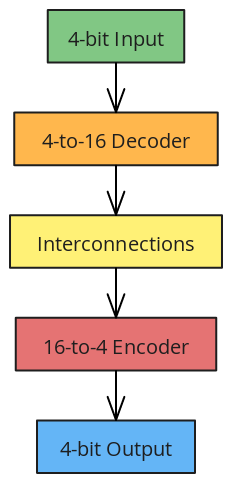
\includegraphics[width=0.4\linewidth]{flow.png}
    \caption{Flowchart of the system}
    \label{fig:flowchart}
\end{figure}

\noindent We follow these steps to implement each component:

\begin{enumerate}[label = (\arabic*)]
    \item 4-16 Decoder:Create a new VHDL file named decoder.vhd. Write the VHDL code to implement a 4-16 decoder that takes a 4-bit input and generates 16 output signals, each corresponding to a unique input combination. Compile the file to ensure correctness and generate the symbol for reuse.

          \begin{lstlisting}[language = VHDL]
LIBRARY IEEE;  
USE IEEE.STD_LOGIC_1164.ALL;  
  
ENTITY Decoder16 IS  
    PORT (  
        E : IN STD_LOGIC;                     -- Enable signal  
        A : IN STD_LOGIC_VECTOR (3 DOWNTO 0); -- 4-bit input  
        Y : OUT STD_LOGIC_VECTOR (15 DOWNTO 0) -- 16-bit output  
    );  
	END Decoder16;  
	  
	ARCHITECTURE Behavioral OF Decoder16 IS  
	BEGIN  
	    PROCESS (E, A)  
	    BEGIN  
	        IF (E = '0') THEN -- Disabled state  
	            Y <= (OTHERS => '0'); -- All output bits are '0'  
	        ELSE  
	            CASE A IS -- Enabled state  
	                WHEN "0000" => Y <= "0000000000000001";  
	                WHEN "0001" => Y <= "0000000000000010";  
	                WHEN "0010" => Y <= "0000000000000100";  
	                WHEN "0011" => Y <= "0000000000001000";  
	                WHEN "0100" => Y <= "0000000000010000";  
	                WHEN "0101" => Y <= "0000000000100000";  
	                WHEN "0110" => Y <= "0000000001000000";  
	                WHEN "0111" => Y <= "0000000010000000";  
	                WHEN "1000" => Y <= "0000000100000000";  
	                WHEN "1001" => Y <= "0000001000000000";  
	                WHEN "1010" => Y <= "0000010000000000";  
	                WHEN "1011" => Y <= "0000100000000000";  
	                WHEN "1100" => Y <= "0001000000000000";  
	                WHEN "1101" => Y <= "0010000000000000";  
	                WHEN "1110" => Y <= "0100000000000000";  
	                WHEN "1111" => Y <= "1000000000000000";  
	                WHEN OTHERS => NULL;  
	            END CASE;  
	        END IF;  
	    END PROCESS;  
	END Behavioral;  


\end{lstlisting}

          \begin{figure}[H]
              \centering
              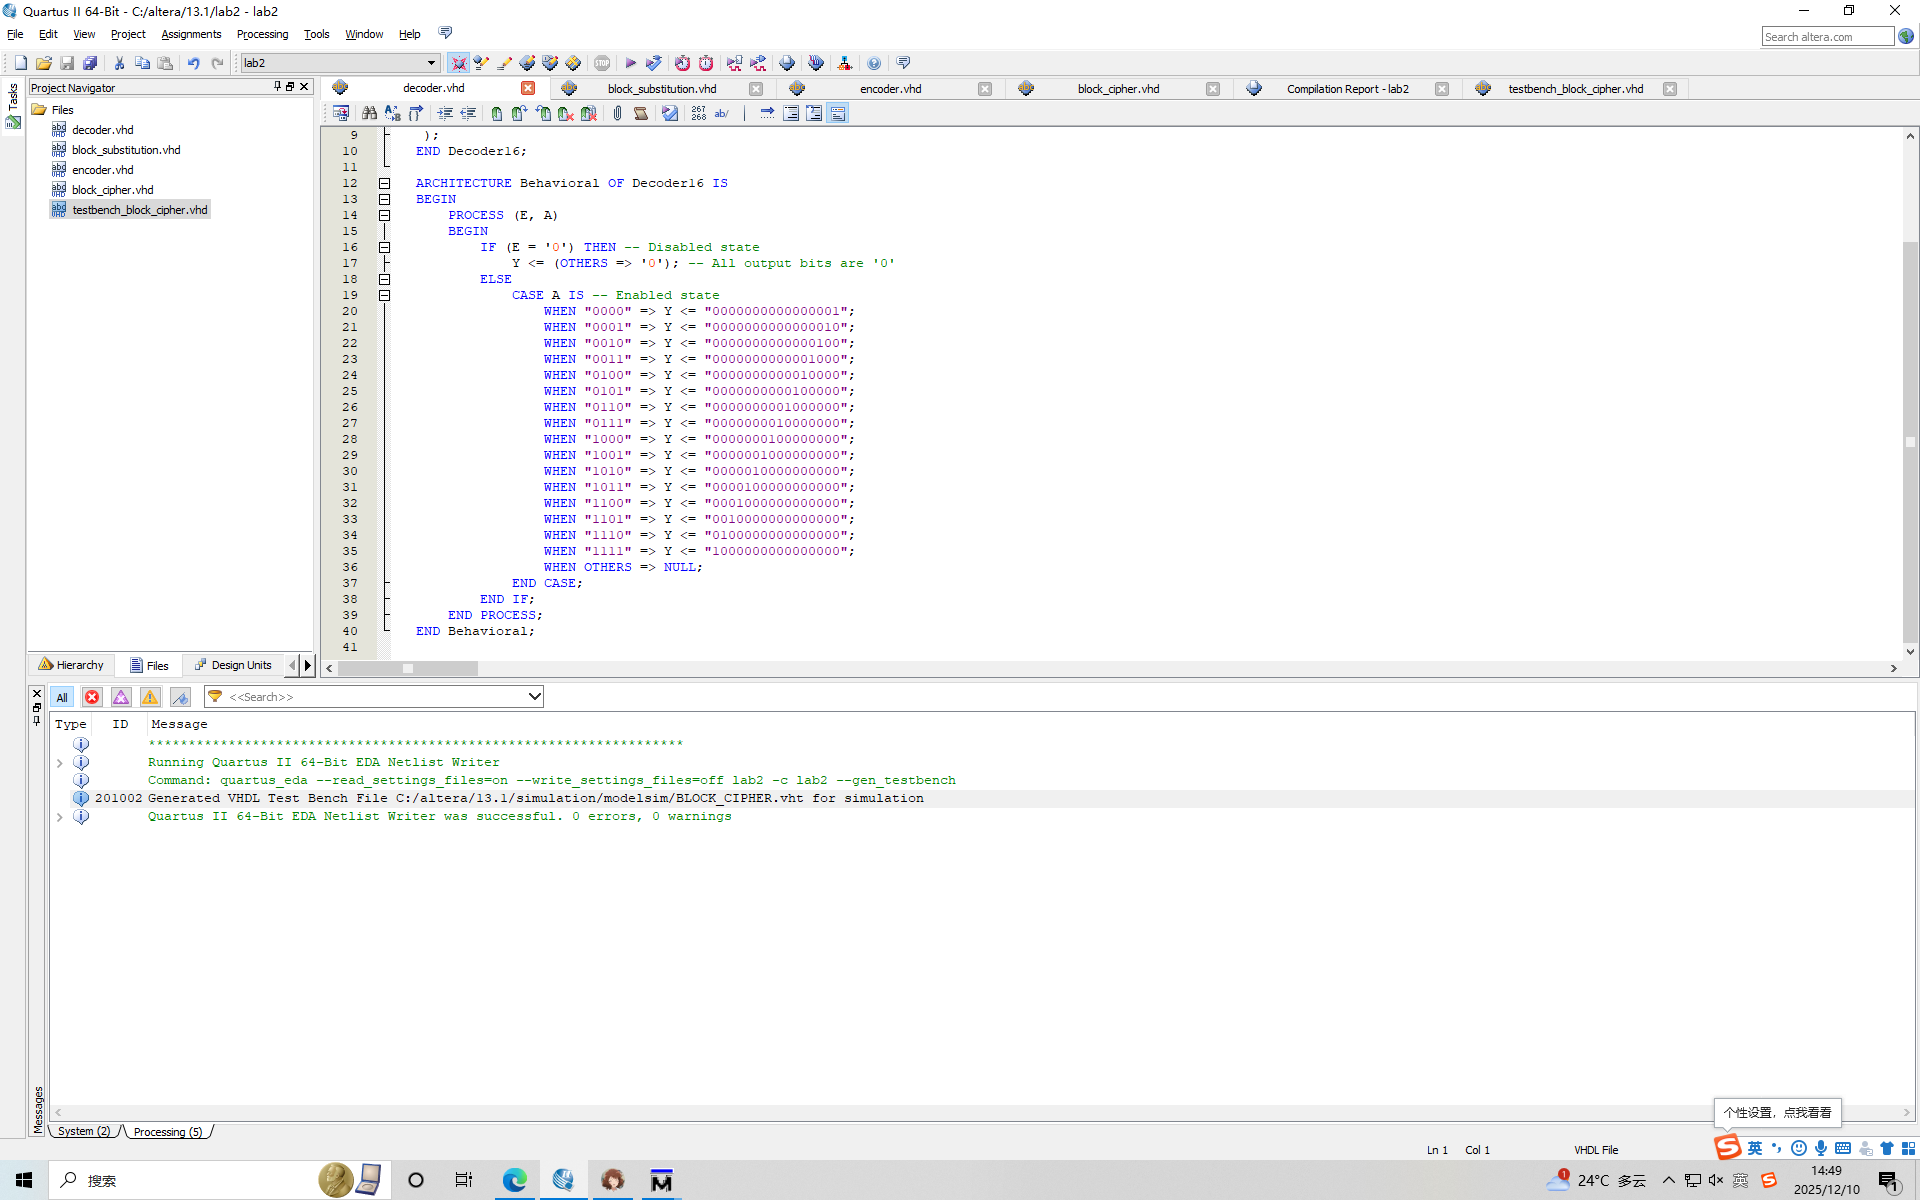
\includegraphics[width=1\linewidth]{decoder.png}
              \caption{4-16 Encoder}
              \label{fig:encoder-164}
          \end{figure}

    \item Block Substitution Module:Create a new VHDL file named block\_substitution.vhd. Implement a substitution logic where each 16-bit input string is mapped to a unique 16-bit output string. For example, input 0000 maps to output 14. Save and compile the file. Generate the symbol for use in the encryption system.

          \begin{lstlisting}[language = VHDL]
LIBRARY IEEE;  
USE IEEE.STD_LOGIC_1164.ALL;  
  
ENTITY CIPHER16 IS  
    PORT (  
        E : IN STD_LOGIC;                     -- Enable signal  
        A : IN STD_LOGIC_VECTOR (15 DOWNTO 0); -- 16-bit input  
        Y : OUT STD_LOGIC_VECTOR (15 DOWNTO 0) -- 16-bit output  
    );  
END CIPHER16;  
  
ARCHITECTURE Behavioral OF CIPHER16 IS  
BEGIN  
    PROCESS (E, A)  
    BEGIN  
        IF (E = '0') THEN -- Disabled state  
            Y <= (OTHERS => '0'); -- All output bits are '0'  
        ELSE  
            CASE A IS -- Enabled state  
                WHEN "0000000000000001" => Y <= "0100000000000000";  
                WHEN "0000000000000010" => Y <= "0000000000010000";  
                WHEN "0000000000000100" => Y <= "0010000000000000";  
                WHEN "0000000000001000" => Y <= "0000000000000010";  
                WHEN "0000000000010000" => Y <= "0000000000000100";  
                WHEN "0000000000100000" => Y <= "1000000000000000";  
                WHEN "0000000001000000" => Y <= "0000100000000000";  
                WHEN "0000000010000000" => Y <= "0000000100000000";  
                WHEN "0000000100000000" => Y <= "0000000000001000";  
                WHEN "0000001000000000" => Y <= "0000010000000000";  
                WHEN "0000010000000000" => Y <= "0000000001000000";  
                WHEN "0000100000000000" => Y <= "0001000000000000";  
                WHEN "0001000000000000" => Y <= "0000000000100000";  
                WHEN "0010000000000000" => Y <= "1000000000000000";  
                WHEN "0100000000000000" => Y <= "0000000000100000";  
                WHEN "1000000000000000" => Y <= "0000000010000000";  
                WHEN OTHERS => NULL; -- Default case  
            END CASE;  
        END IF;  
    END PROCESS;  
	END Behavioral; 

    \end{lstlisting}

          \begin{figure}[H]
              \centering
              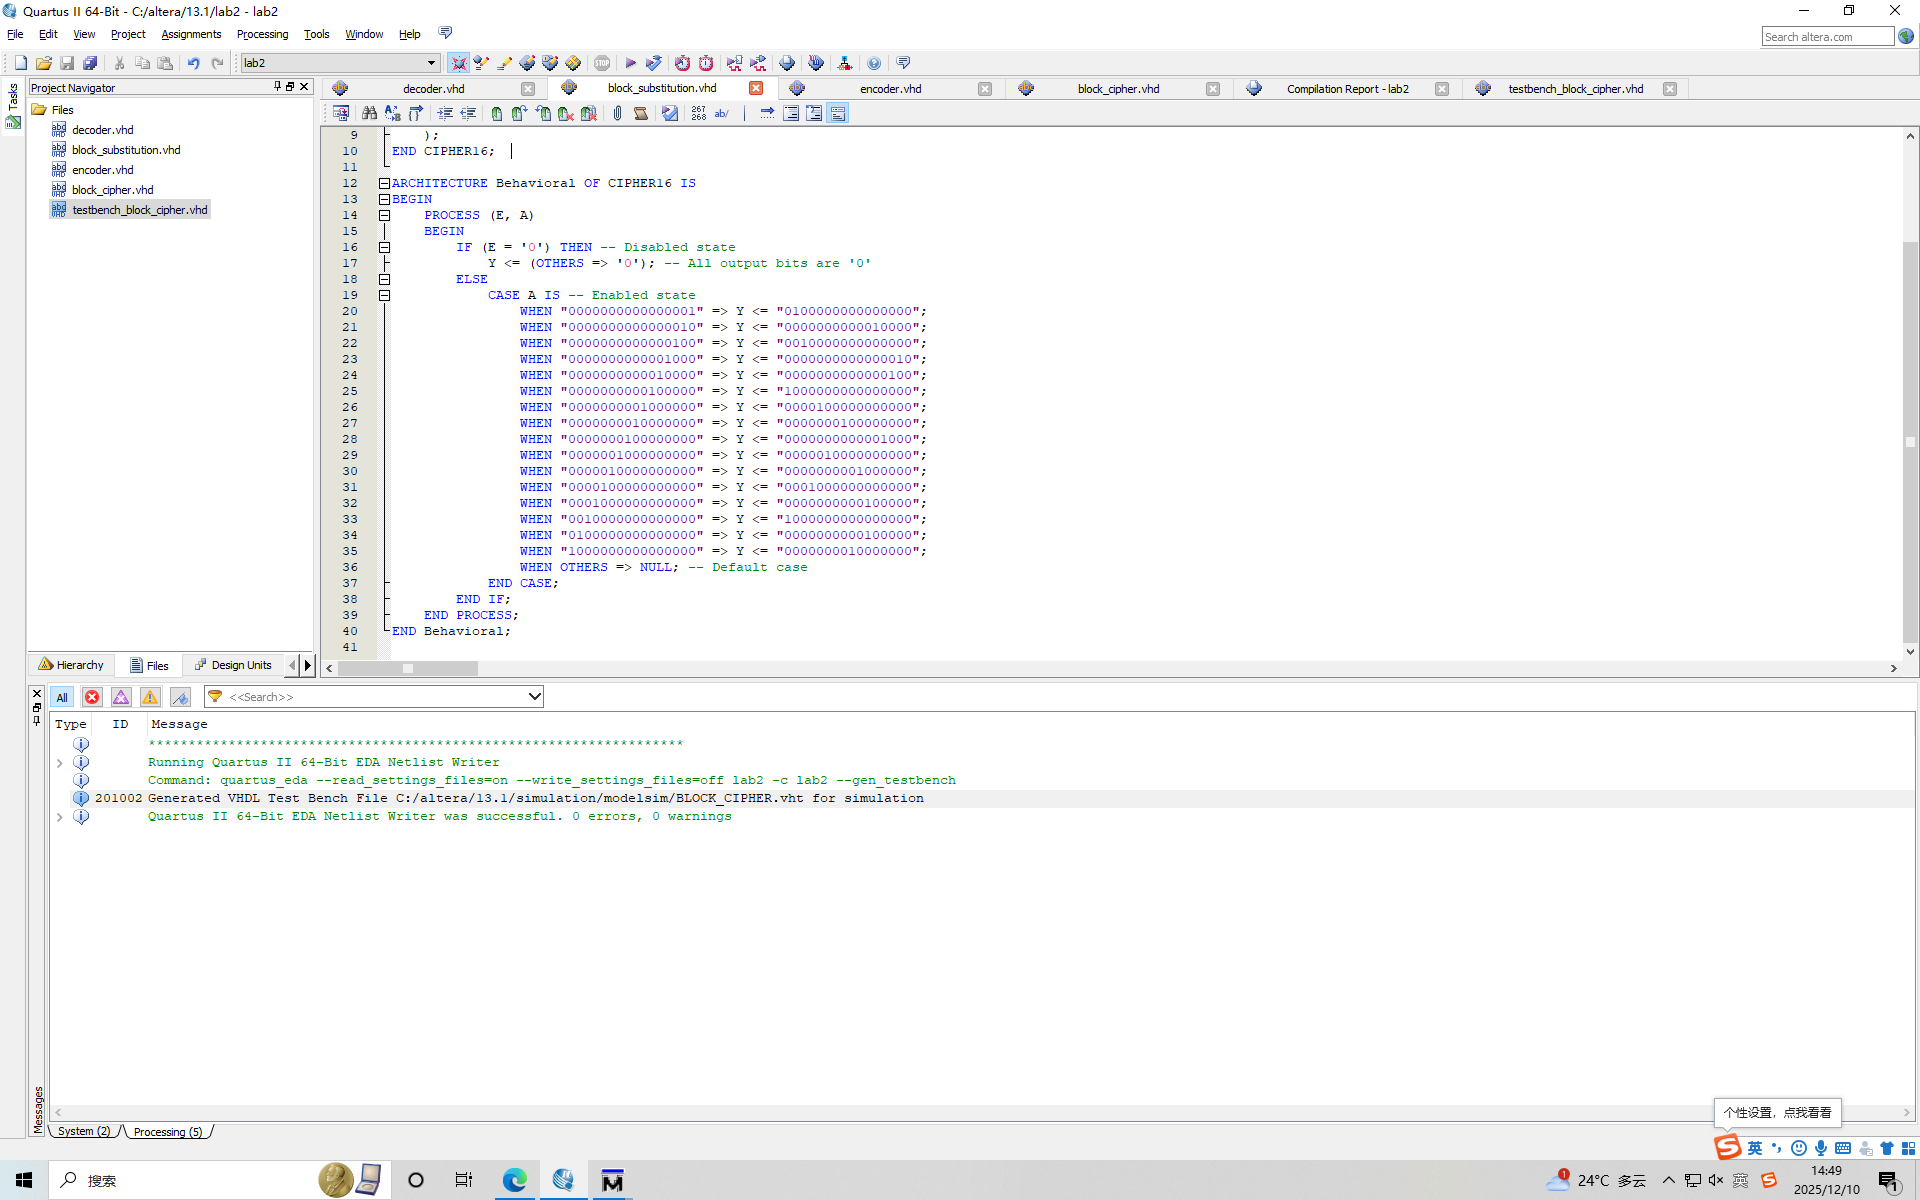
\includegraphics[width=1\linewidth]{substitution.png}
              \caption{Block Substitution Module}
              \label{fig:substitution-module}
          \end{figure}

    \item 16-4 Encoder:Create a VHDL file named encoder.vhd. Implement logic to compress 16 input signals into a corresponding 4-bit output, effectively reversing the decoding process. Compile the file and generate its symbol.    \begin{lstlisting}[language = VHDL]
LIBRARY IEEE;  
USE IEEE.STD_LOGIC_1164.ALL;  
  
ENTITY Encoder16 IS  
    PORT (  
        E : IN STD_LOGIC;                      -- Enable signal  
        A : IN STD_LOGIC_VECTOR (15 DOWNTO 0); -- 16-bit input  
        Y : OUT STD_LOGIC_VECTOR (3 DOWNTO 0)  -- 4-bit output  
    );  
END Encoder16;  
  
ARCHITECTURE Behavioral OF Encoder16 IS  
BEGIN  
    PROCESS (E, A)  
    BEGIN  
        IF (E = '0') THEN -- Disabled state  
            Y <= "ZZZZ"; -- Undefined state  
        ELSE  
            CASE A IS -- Enabled state  
                WHEN "0000000000000001" => Y <= "0000";  
                WHEN "0000000000000010" => Y <= "0001";  
                WHEN "0000000000000100" => Y <= "0010";  
                WHEN "0000000000001000" => Y <= "0011";  
                WHEN "0000000000010000" => Y <= "0100";  
                WHEN "0000000000100000" => Y <= "0101";  
                WHEN "0000000001000000" => Y <= "0110";  
                WHEN "0000000010000000" => Y <= "0111";  
                WHEN "0000000100000000" => Y <= "1000";  
                WHEN "0000001000000000" => Y <= "1001";  
                WHEN "0000010000000000" => Y <= "1010";  
                WHEN "0000100000000000" => Y <= "1011";  
                WHEN "0001000000000000" => Y <= "1100";  
                WHEN "0010000000000000" => Y <= "1101";  
                WHEN "0100000000000000" => Y <= "1110";  
                WHEN "1000000000000000" => Y <= "1111";  
                WHEN OTHERS => NULL; -- Default case  
            END CASE;  
        END IF;  
    END PROCESS;  
END Behavioral;  

    \end{lstlisting}
          \begin{figure}[H]
              \centering
              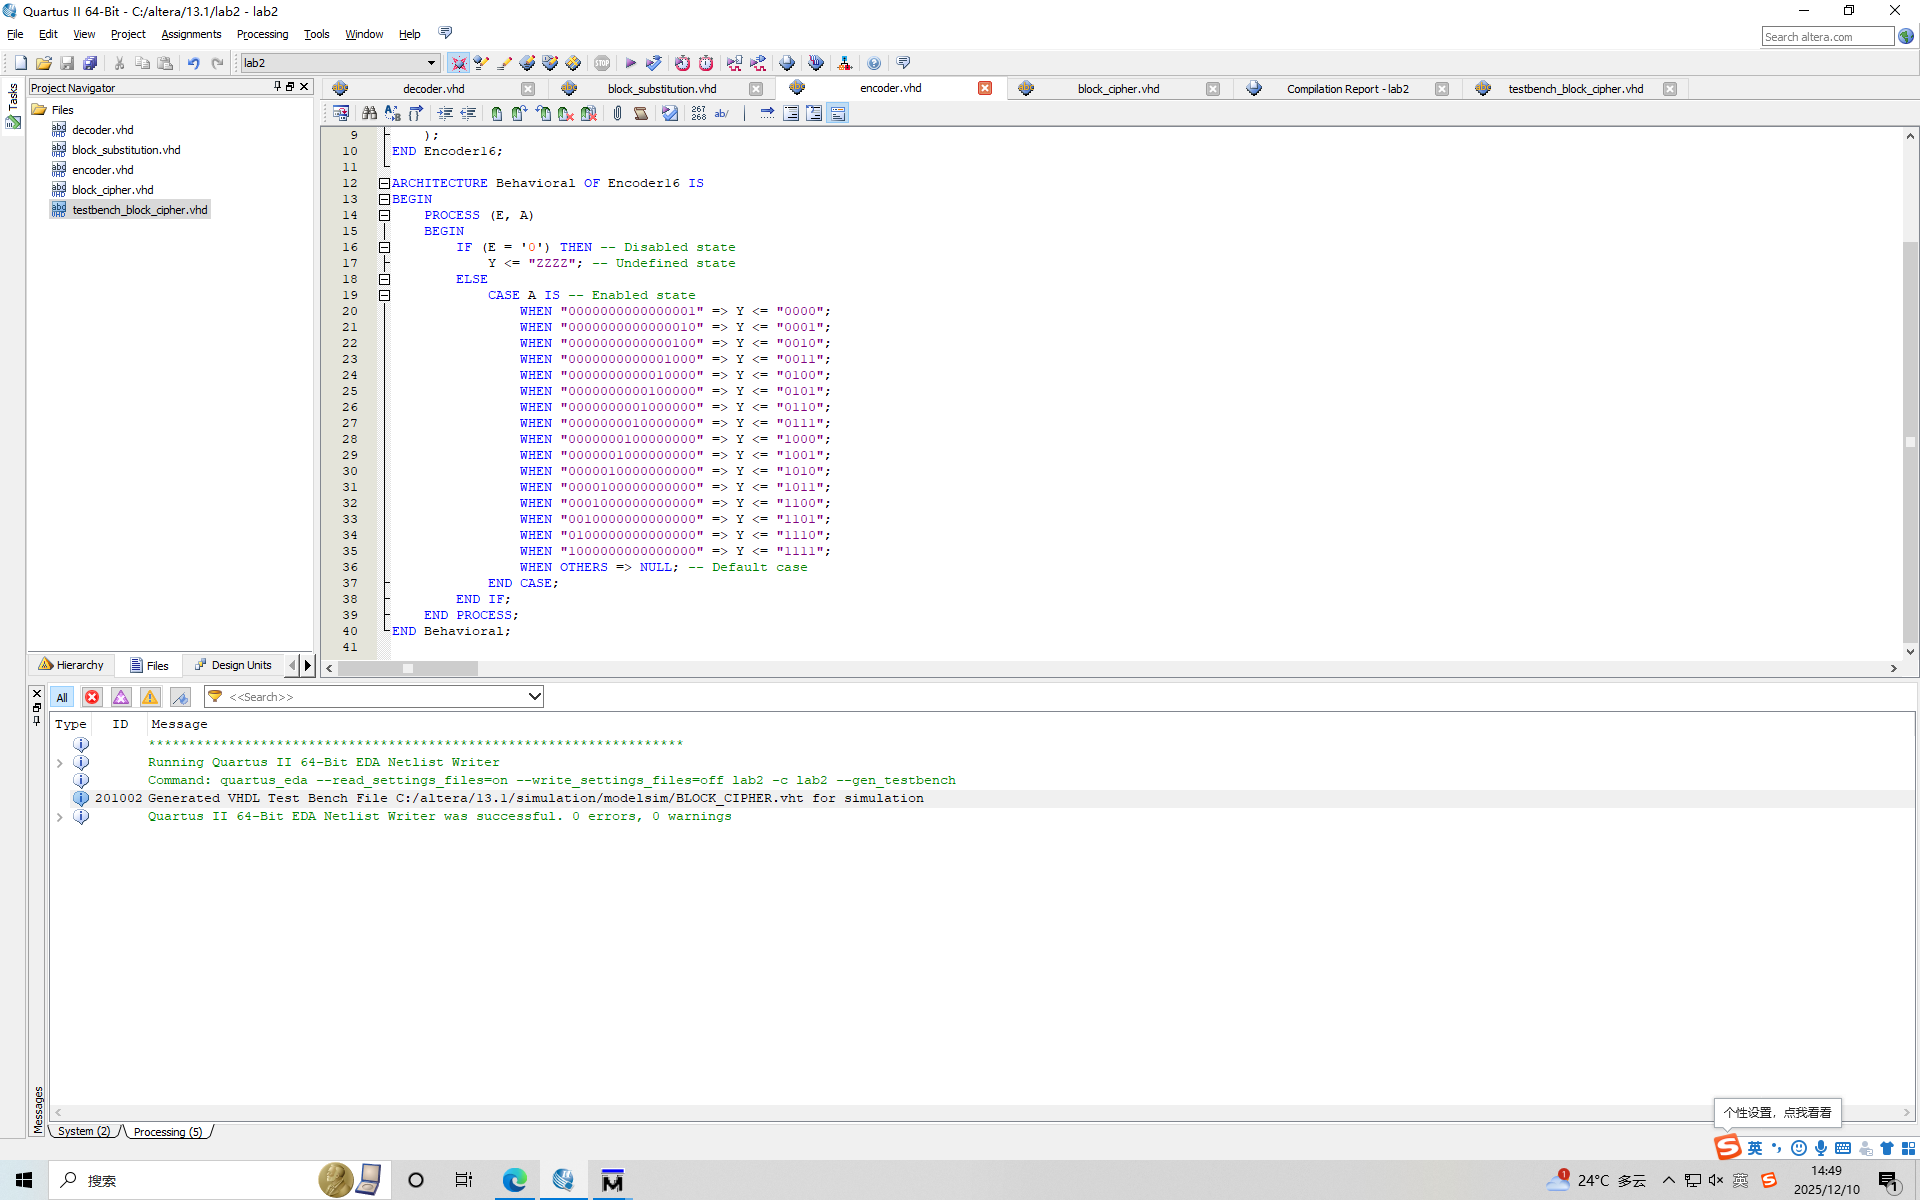
\includegraphics[width=1\linewidth]{encoder.png}
              \caption{16-4 Encoder}
              \label{fig:arch-ed}
          \end{figure}

\end{enumerate}

\subsection{Integrate the Data Encryption System}
\renewcommand{\theenumi}{(\arabic{enumi})}
\begin{enumerate}
    \item Create a top-level VHDL file named data\_encryption.vhd.
    \item Instantiate the decoder, block\_substitution, and encoder components within this file. Connect their inputs and outputs to implement the complete 4-bit data encryption system.
    \item Compile the top-level file to check for errors and generate the system's symbol file.
    \item Generate the RTL (Register Transfer Level) view in Quartus II and save the graphical representation of the system.
\end{enumerate}
\begin{lstlisting}[language=VHDL]
LIBRARY IEEE;  
USE IEEE.STD_LOGIC_1164.ALL;  
  
ENTITY BLOCK_CIPHER IS  
    PORT (  
        E : IN STD_LOGIC;                       -- Enable signal  
        A : IN STD_LOGIC_VECTOR(3 DOWNTO 0);    -- 4-bit input  
        Y : OUT STD_LOGIC_VECTOR(3 DOWNTO 0)    -- 4-bit output  
    );  
	END BLOCK_CIPHER;  
	  
	ARCHITECTURE Behavioral OF BLOCK_CIPHER IS  
	  
	    -- Component declaration for DECODER16  
	    COMPONENT DECODER16  
	        PORT (  
	            E : IN STD_LOGIC;                    -- Enable signal  
	            A : IN STD_LOGIC_VECTOR(3 DOWNTO 0); -- 4-bit input  
	            Y : OUT STD_LOGIC_VECTOR(15 DOWNTO 0) -- 16-bit output  
	        );  
	    END COMPONENT;  
	  
	    -- Component declaration for ENCODER16  
	    COMPONENT ENCODER16  
	        PORT (  
	            E : IN STD_LOGIC;                     -- Enable signal  
	            A : IN STD_LOGIC_VECTOR(15 DOWNTO 0); -- 16-bit input  
	            Y : OUT STD_LOGIC_VECTOR(3 DOWNTO 0)  -- 4-bit output  
	        );  
	    END COMPONENT;  
	  
	    -- Component declaration for CIPHER16  
	    COMPONENT CIPHER16  
	        PORT (  
	            E : IN STD_LOGIC;                     -- Enable signal  
	            A : IN STD_LOGIC_VECTOR(15 DOWNTO 0); -- 16-bit input  
	            Y : OUT STD_LOGIC_VECTOR(15 DOWNTO 0) -- 16-bit output  
	        );  
	    END COMPONENT;  
	  
	    -- Signal declarations  
	    SIGNAL DE_SIG : STD_LOGIC_VECTOR(15 DOWNTO 0);   
	    SIGNAL CI_SIG : STD_LOGIC_VECTOR(15 DOWNTO 0); 
	  
	BEGIN  
	    -- Instance of DECODER16  
	    U1 : DECODER16  
	        PORT MAP (  
	            E => E,  
	            A => A(3 DOWNTO 0),  
	            Y => DE_SIG(15 DOWNTO 0)  
	        );  
	  
	    -- Instance of CIPHER16  
	    U2 : CIPHER16  
	        PORT MAP (  
	            E => E,  
	            A => DE_SIG(15 DOWNTO 0),  
	            Y => CI_SIG(15 DOWNTO 0)  
	        );  
	  
	    -- Instance of ENCODER16  
	    U3 : ENCODER16  
	        PORT MAP (  
	            E => E,  
	            A => CI_SIG(15 DOWNTO 0),  
	            Y => Y(3 DOWNTO 0)  
	        );  
	  
	END Behavioral; 

\end{lstlisting}

\begin{figure}[H]
    \centering
    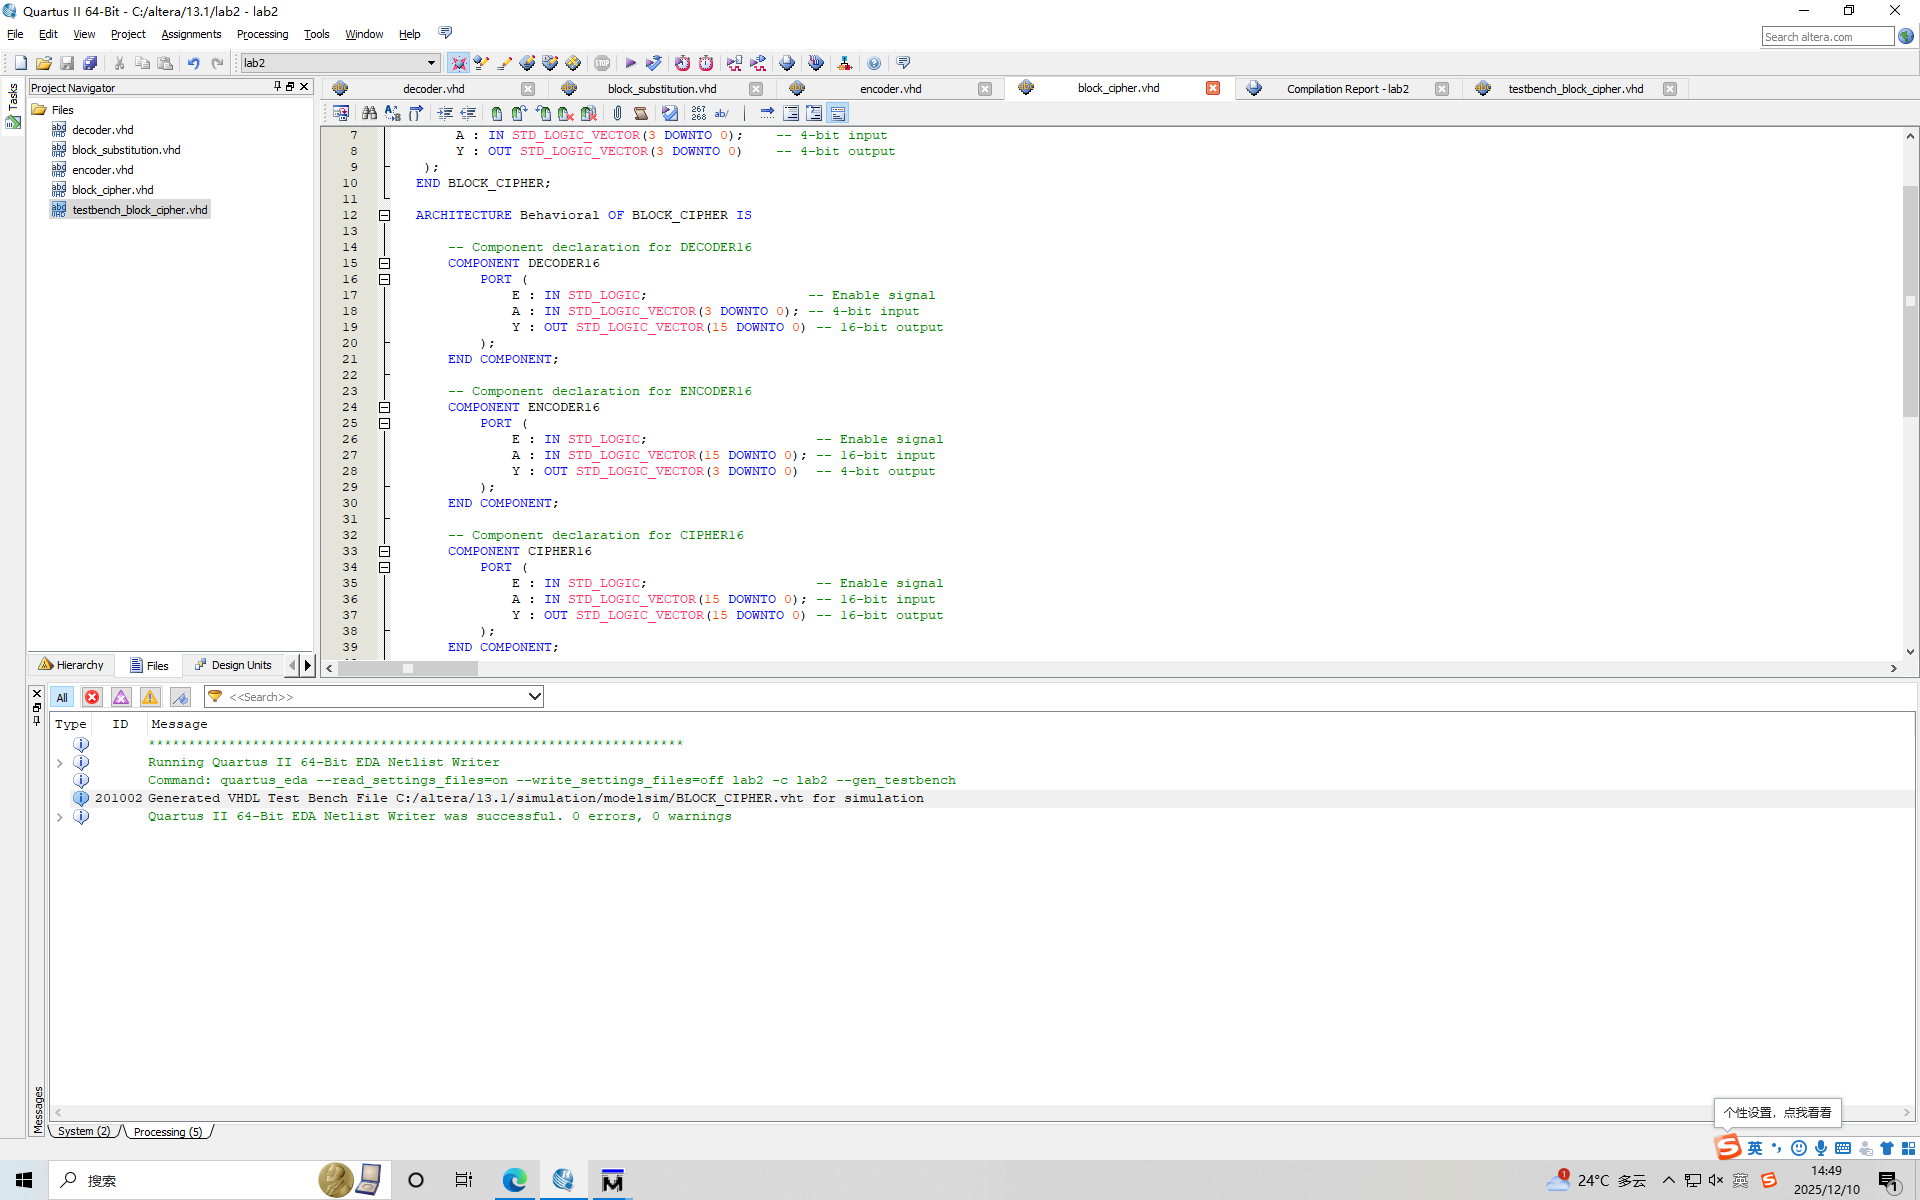
\includegraphics[width=1\linewidth]{cipher.png}
    \caption{CIPHER16 Component}
    \label{fig:cipher16-component}
\end{figure}

\subsection{Testbench Design}
\renewcommand{\theenumi}{(\arabic{enumi})}
\begin{enumerate}
    \item Create a testbench file named testbench\_block\_cipher.vhd.
    \item 	Design the testbench to provide all possible 4-bit input combinations (0000 to 1111) to the encryption system.
    \item Add appropriate clock and signal initialization to simulate the system's behavior.
    \item Compile the testbench to verify its functionality.
\end{enumerate}

\begin{lstlisting}[language=VHDL]
LIBRARY ieee;  
USE ieee.std_logic_1164.ALL;  
  
ENTITY BLOCK_CIPHER_vhd_tst IS  
END BLOCK_CIPHER_vhd_tst;  
  
ARCHITECTURE BLOCK_CIPHER_arch OF BLOCK_CIPHER_vhd_tst IS  
  
    -- Signal Declarations  
	    SIGNAL A : STD_LOGIC_VECTOR(3 DOWNTO 0); -- Input signal A  
	    SIGNAL E : STD_LOGIC;                    -- Enable signal E  
	    SIGNAL Y : STD_LOGIC_VECTOR(3 DOWNTO 0); -- Output signal Y  
	  
	    -- Component Declaration for BLOCK_CIPHER  
	    COMPONENT BLOCK_CIPHER  
	        PORT (  
	            A : IN STD_LOGIC_VECTOR(3 DOWNTO 0); -- 4-bit input  
	            E : IN STD_LOGIC;                    -- Enable signal  
	            Y : OUT STD_LOGIC_VECTOR(3 DOWNTO 0) -- 4-bit output  
	        );  
	    END COMPONENT;  
	  
	BEGIN  
	  
	    -- Instantiating BLOCK_CIPHER Component  
	    i1 : BLOCK_CIPHER  
	        PORT MAP (  
	            A => A,  
	            E => E,  
	            Y => Y  
	        );  
	  
	    -- Test Process for Initialization  
	    init : PROCESS  
	    BEGIN  
	        -- Initialize enable and input signals  
	        E <= '0';  
	        A <= "0000";  
	        WAIT FOR 50 ns;  
	  
	        E <= '1';  
	        WAIT FOR 50 ns;  
	  
	        -- Apply test inputs to signal A  
	        A <= "0001";  
	        WAIT FOR 50 ns;  
	  
	        A <= "0010";  
	        WAIT FOR 50 ns;  
	  
	        A <= "0011";  
	        WAIT FOR 50 ns;  
	  
	        A <= "0100";  
	        WAIT FOR 50 ns;  
	  
	        A <= "0101";  
	        WAIT FOR 50 ns;  
	  
	        A <= "0110";  
	        WAIT FOR 50 ns;  
	  
	        A <= "0111";  
	        WAIT FOR 50 ns;  
	  
	        A <= "1000";  
	        WAIT FOR 50 ns;  
	  
	        A <= "1001";  
	        WAIT FOR 50 ns;  
	  
	        A <= "1010";  
	        WAIT FOR 50 ns;  
	  
	        A <= "1011";  
	        WAIT FOR 50 ns;  
	  
	        A <= "1100";  
	        WAIT FOR 50 ns;  
	  
	        A <= "1101";  
	        WAIT FOR 50 ns;  
	  
	        A <= "1110";  
	        WAIT FOR 50 ns;  
	  
	        A <= "1111";  
	        WAIT;  
	  
	    END PROCESS init;  
	  
	     
	    always : PROCESS  
	    BEGIN  
 
	        WAIT;  
	    END PROCESS always;  
	  
	END BLOCK_CIPHER_arch;  

\end{lstlisting}

\begin{figure}[H]
    \centering
    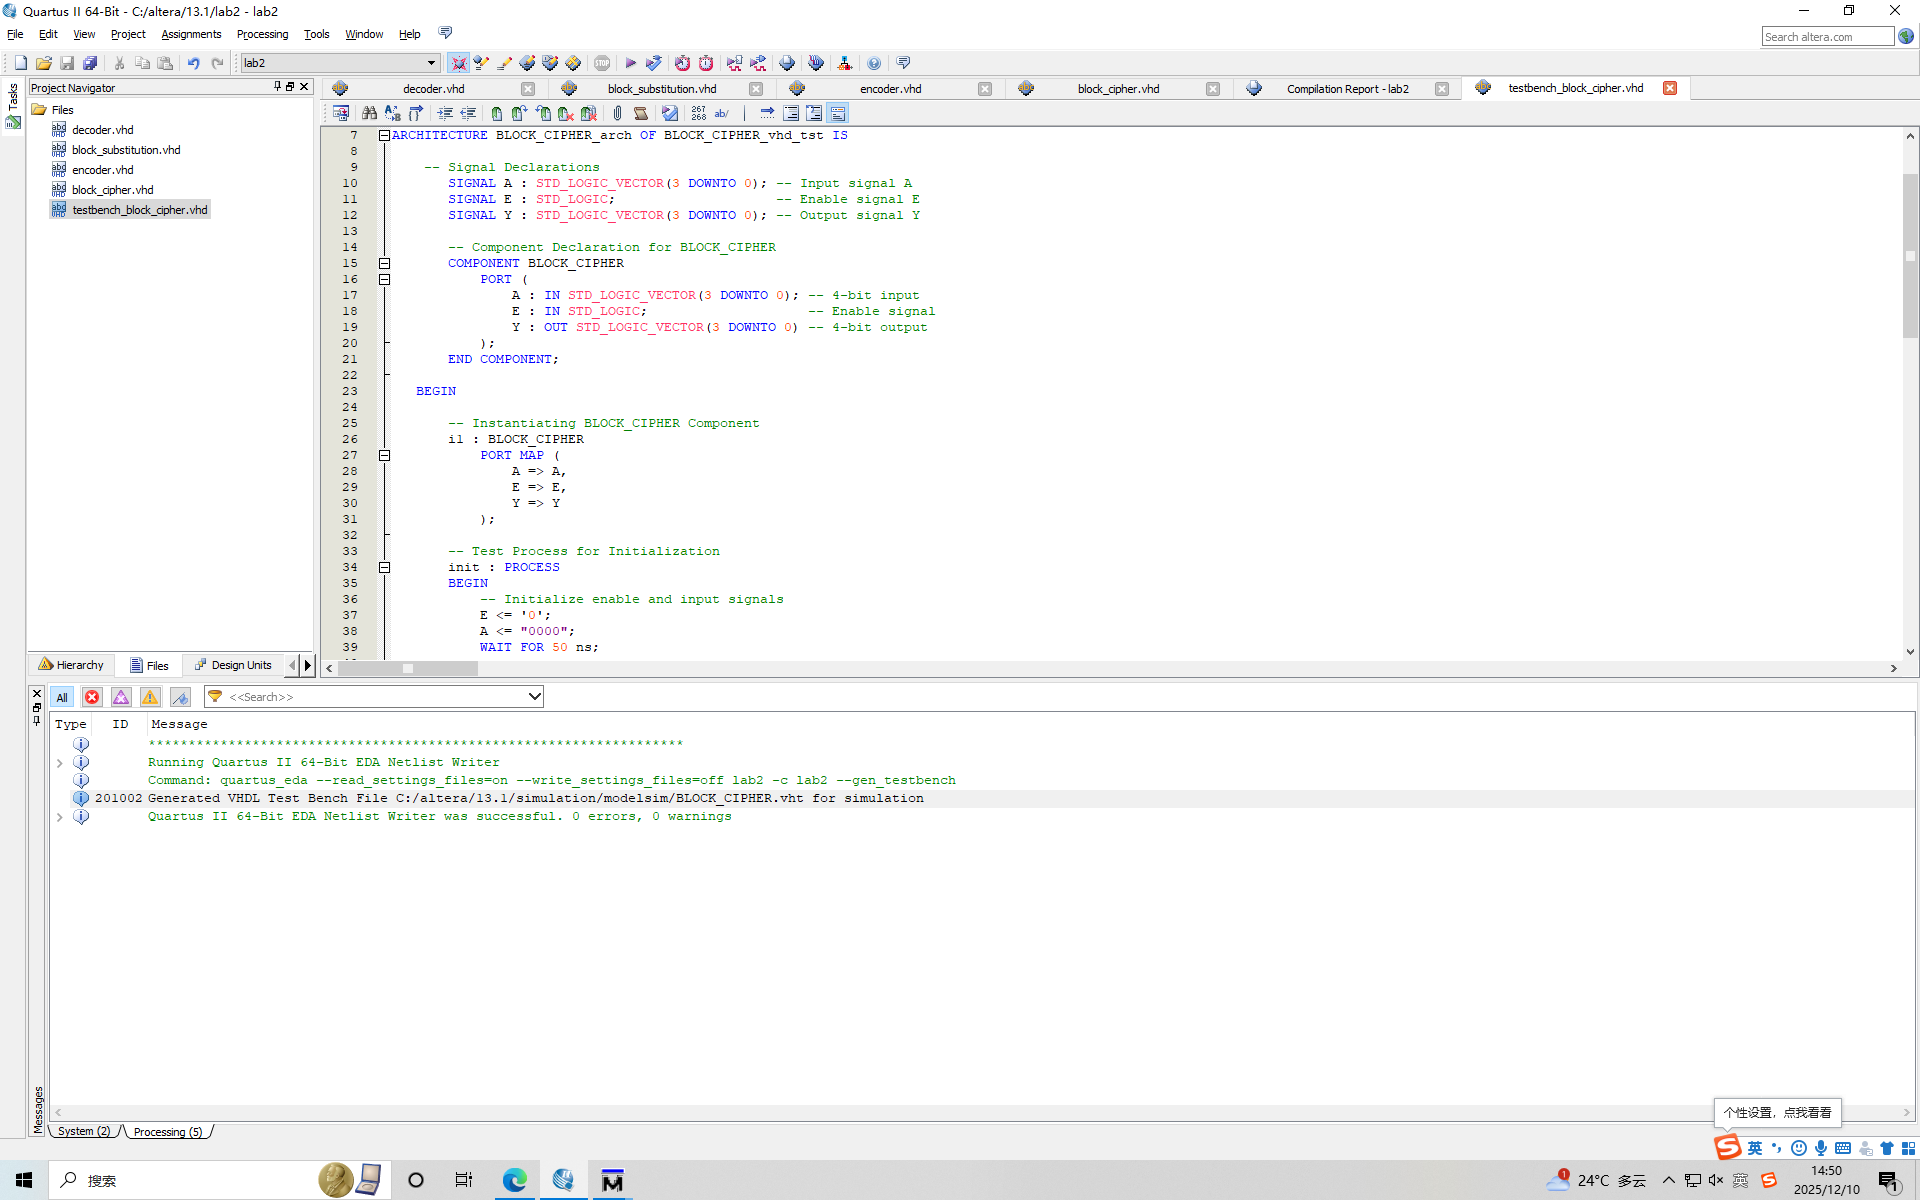
\includegraphics[width=1\linewidth]{testbench.png}
    \caption{Testbench Module}
    \label{fig:testbench-module}
\end{figure}


\subsection{Simulation}
\begin{enumerate}
    \item Open Modelsim and set up the simulation environment.
    \item Add the compiled encryption system and its testbench files to the Modelsim project.
    \item Simulate the design by applying all possible inputs through the testbench. Observe the output waveforms for each input combination.
    \item Record the simulation waveforms and save the results for inclusion in the report.
\end{enumerate}


\subsection{Data Decryption System}
\noindent Design a 4-bit decryption system to reverse the encryption process. Implement the decryption logic by designing inverse components for substitution and encoding. Test the decryption system using a similar testbench.

\begin{lstlisting}[language=VHDL]
LIBRARY IEEE;  
USE IEEE.STD_LOGIC_1164.ALL;  
  
ENTITY CIPHER16 IS  
    PORT (  
        E : IN STD_LOGIC;                     -- Enable signal  
        A : IN STD_LOGIC_VECTOR (15 DOWNTO 0); -- 16-bit input  
        Y : OUT STD_LOGIC_VECTOR (15 DOWNTO 0) -- 16-bit output  
    );  
END CIPHER16;  
  
ARCHITECTURE Behavioral OF CIPHER16 IS  
BEGIN  
    PROCESS (E, A)  
    BEGIN  
        IF (E = '0') THEN -- Disabled state  
            Y <= (OTHERS => '0'); -- All output bits are '0'  
        ELSE  
            CASE A IS -- Enabled state  
                WHEN "0100000000000000" => Y <= "0000000000000001";  
                WHEN "0000000000010000" => Y <= "0000000000000010";  
                WHEN "0010000000000000" => Y <= "0000000000000100";  
                WHEN "0000000000000010" => Y <= "0000000000001000";  
                WHEN "0000000000000100" => Y <= "0000000000010000";  
                WHEN "1000000000000000" => Y <= "0000000000100000";  
                WHEN "0000100000000000" => Y <= "0000000001000000";  
                WHEN "0000000100000000" => Y <= "0000000010000000";  
                WHEN "0000000000001000" => Y <= "0000000100000000";  
                WHEN "0000010000000000" => Y <= "0000001000000000";  
                WHEN "0000000001000000" => Y <= "0000010000000000";  
                WHEN "0001000000000000" => Y <= "0000100000000000";  
                WHEN "0000000000100000" => Y <= "0001000000000000";  
                WHEN "1000000000000000" => Y <= "0010000000000000";  
                WHEN "0000000000100000" => Y <= "0100000000000000";  
                WHEN "0000000010000000" => Y <= "1000000000000000";  
                WHEN OTHERS => NULL; -- Default case  
            END CASE;  
        END IF;  
    END PROCESS;  
END Behavioral;  

\end{lstlisting}

\section{Experimental record}
\noindent Below are some records of my second experiment.

\begin{figure}[H]
    \centering
    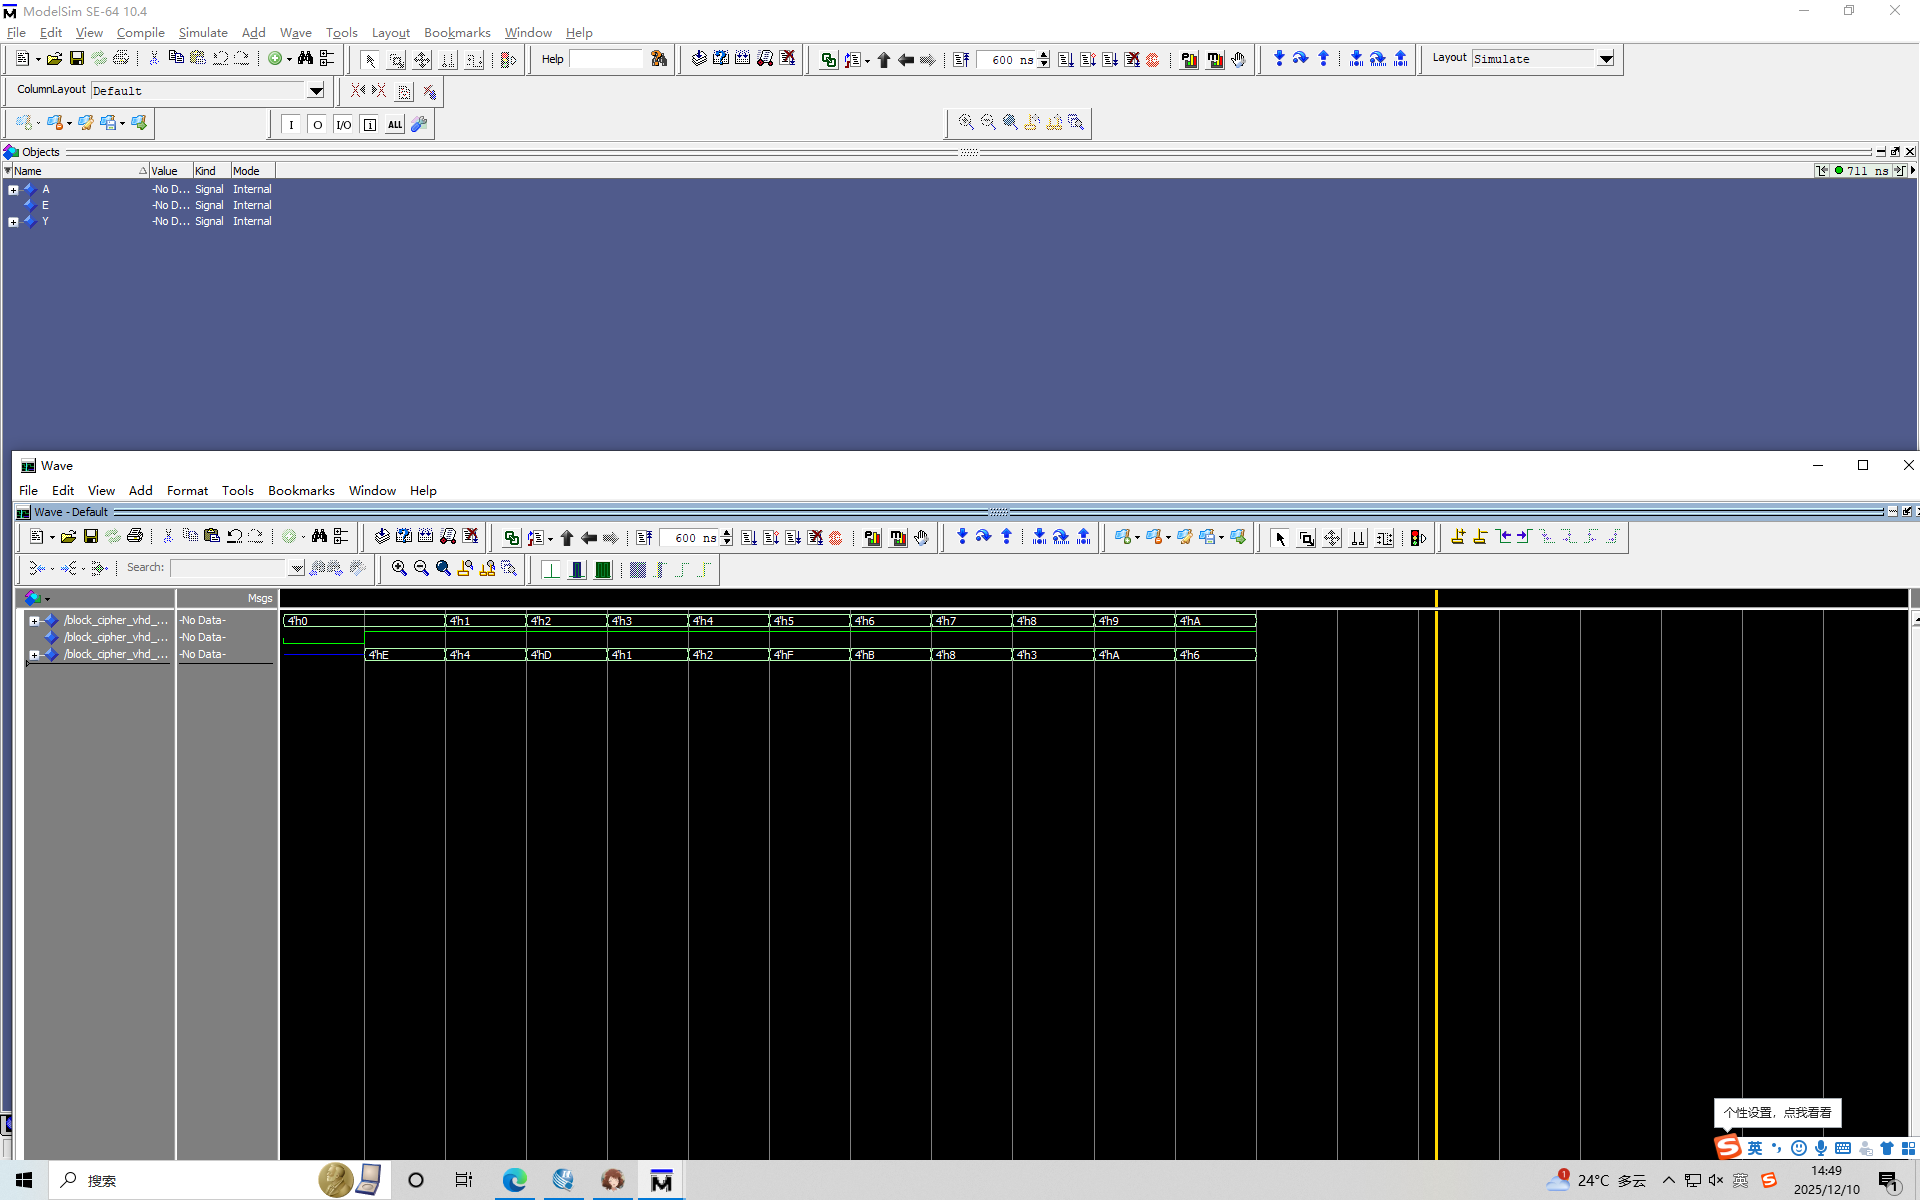
\includegraphics[width=1\linewidth]{encryption.png}
    \caption{Encryption Simulation Waveform (original)}
    \label{fig:wave-orig}
\end{figure}

\begin{figure}[H]
    \centering
    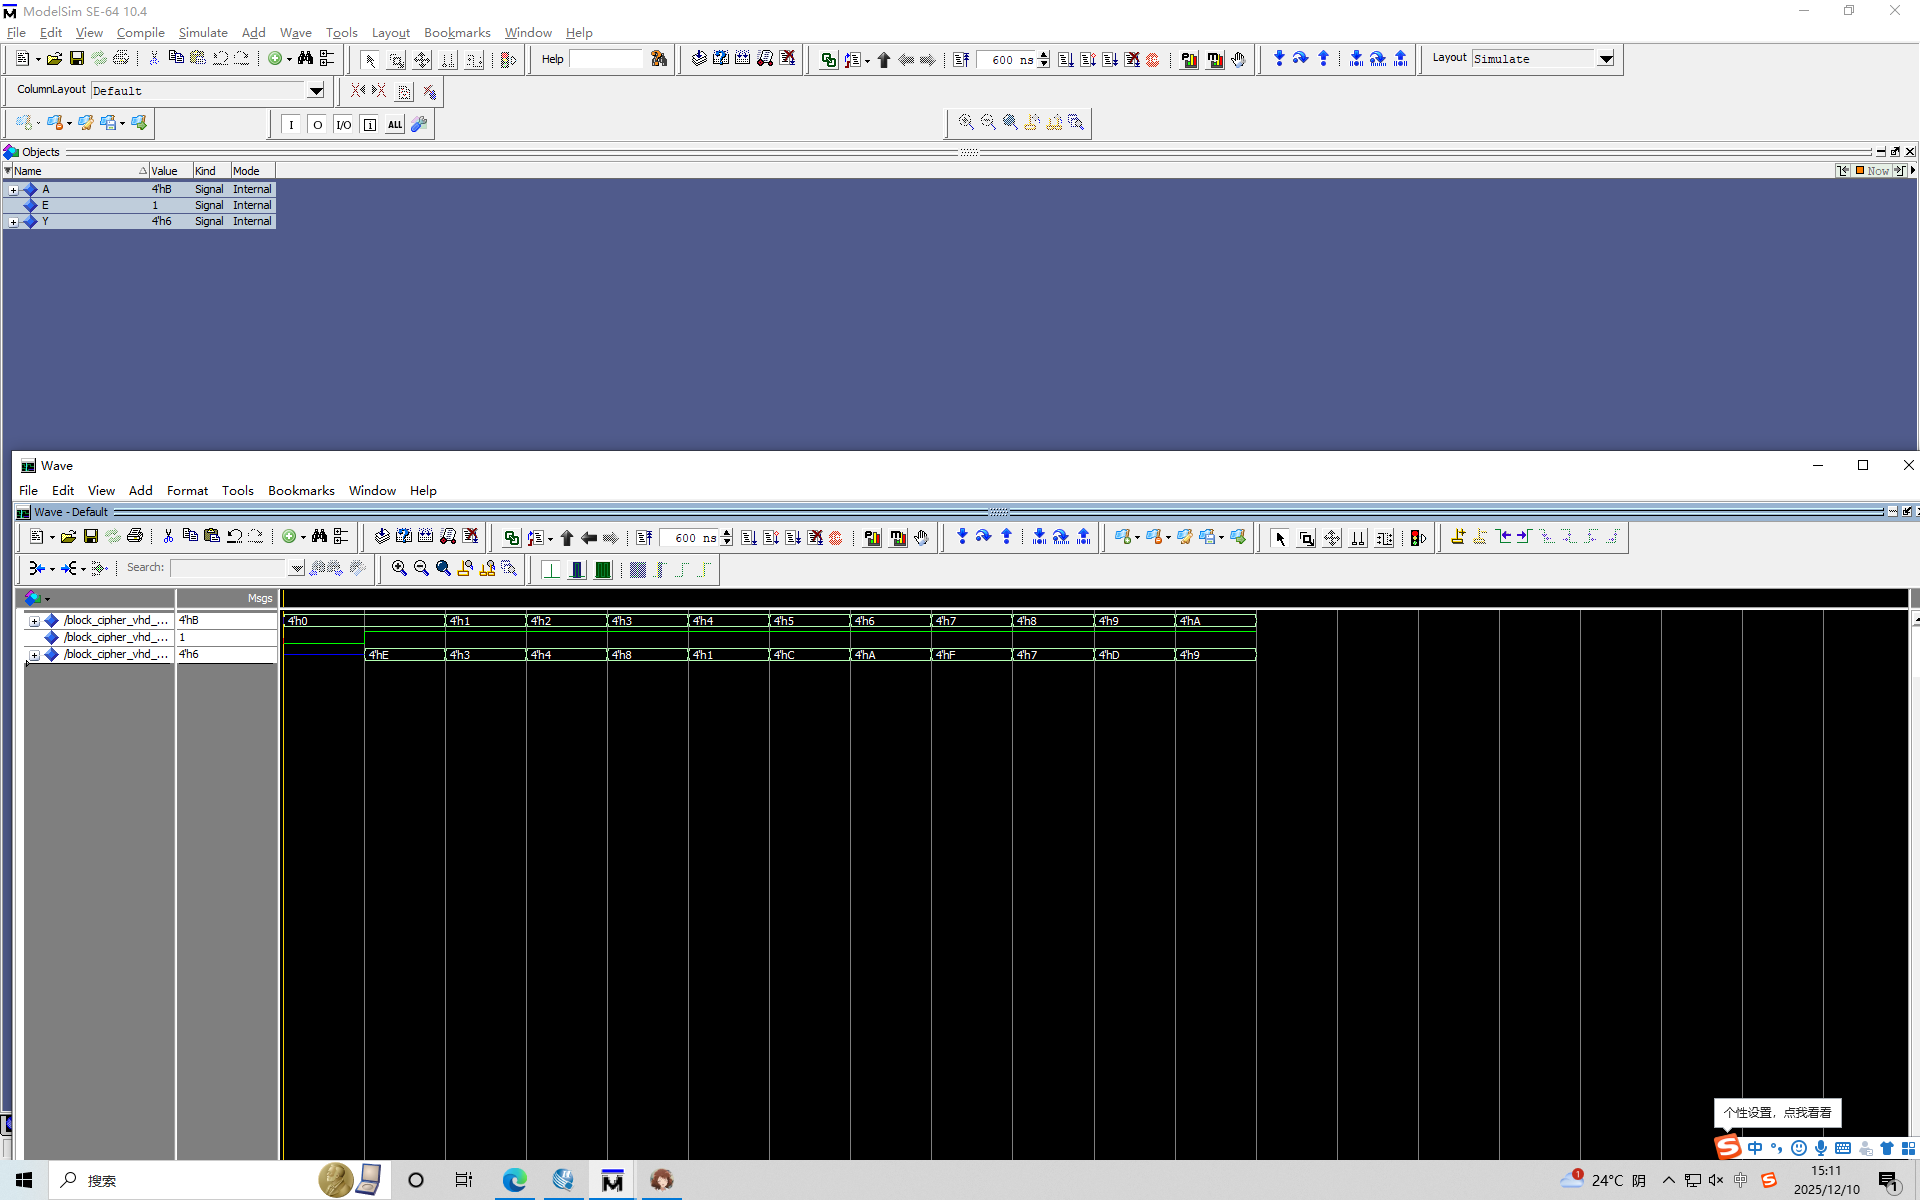
\includegraphics[width=1\linewidth]{decryption.png}
    \caption{DecryptionSimulation Waveform (optional)}
    \label{fig:wave-opt}
\end{figure}
\section{Analysis and discussion}
\subsection{Overall Conclusion}
\noindent The comprehensive simulation of the 4-bit data encryption system convincingly attests to its impeccable functional correctness. It vividly showcases the precise and appropriate transformation of input data as it traverses through the three crucial main components, namely a highly efficient decoder, a sophisticated block substitution module, and a reliable encoder.

\subsection{Function of the System}
\begin{enumerate}
    \item The 4-16 decoder successfully converts the 4-bit input into a 16-bit output, with each bit representing one of the possible input combinations. This transformation aligns with the expected functionality.
    \item The substitution module maps the 16-bit input from the decoder to a different 16-bit string based on the substitution table. This step effectively represents the encryption logic.
    \item The encoder compresses the 16-bit output from the substitution module back into a 4-bit result, maintaining the integrity of the data through the transformation.
\end{enumerate}

\subsection{Explanation of the waveform}
\begin{enumerate}
    \item The propagation of signals through the decoder, substitution module, and encoder occurred without delays or glitches, indicating proper synchronization.
    \item All possible input combinations were tested, and the corresponding outputs matched the expected results based on the substitution logic.

\end{enumerate}

\section{Answers to the question}
\noindent I can't make sure whether the input 776979603 is a sequence or just a number in decimal. So I will take the two cases into my consideration.
\subsection{As sequence(std\_logic\_vector)}
\noindent In such case, we can just generate our answer bit by bit (like BCD code) from the mapping relation.
$$\text{7 7 6 9 7 9 6 0 3} \to \text{8 8 11 10 8 10 11 14 1}$$

\subsection{As a decimal number}
\begin{enumerate}

    \item The decimal input 776979603 is firstly converted to binary(unsigned):\\
          $$776979603 (decimal) = 101110010011111100010010010011 (binary)$$

    \item Pad the binary value to fit into groups of 4 bits,and divide it into 4-bit groups like below:
          $$0010 1110 0100 1111 1100 0100 1001 0011$$

    \item Convert by the system:
          $$ 1101 0000 0010 0111 0101 0010 1010 0001$$

    \item  Convert the combined binary output to decimal:
          $$11010000001001110101001010100001(binary) = 3492237985(decimal)$$

\end{enumerate}
\end{document}
